\documentclass[11pt,a4paper,oneside]{report}

\usepackage{color}
\usepackage{hyperref}

\usepackage{bytefield}
\usepackage[margin=3cm]{geometry}
\usepackage{tabularx}
\usepackage{multirow}   % multiple line rows and columns in tabulars
\usepackage{graphicx}   % required to include images

\title{CWIS Ground Software User Reference Manual}
\author{Olivier Desenfans}

\begin{document}

\maketitle

\tableofcontents

\chapter{Introduction}

This document describes the user interface to communicate with the CWIS Rexus/Bexus experiment.
It is divided in two parts.
The first describes the \emph{ground software}, the GUI (Graphical User Interface) used to visualize data and interact with the experiment.
The second describes the low level serial interface.

\chapter{Ground Software}

\section{Description}

\begin{figure}[!h]
\center
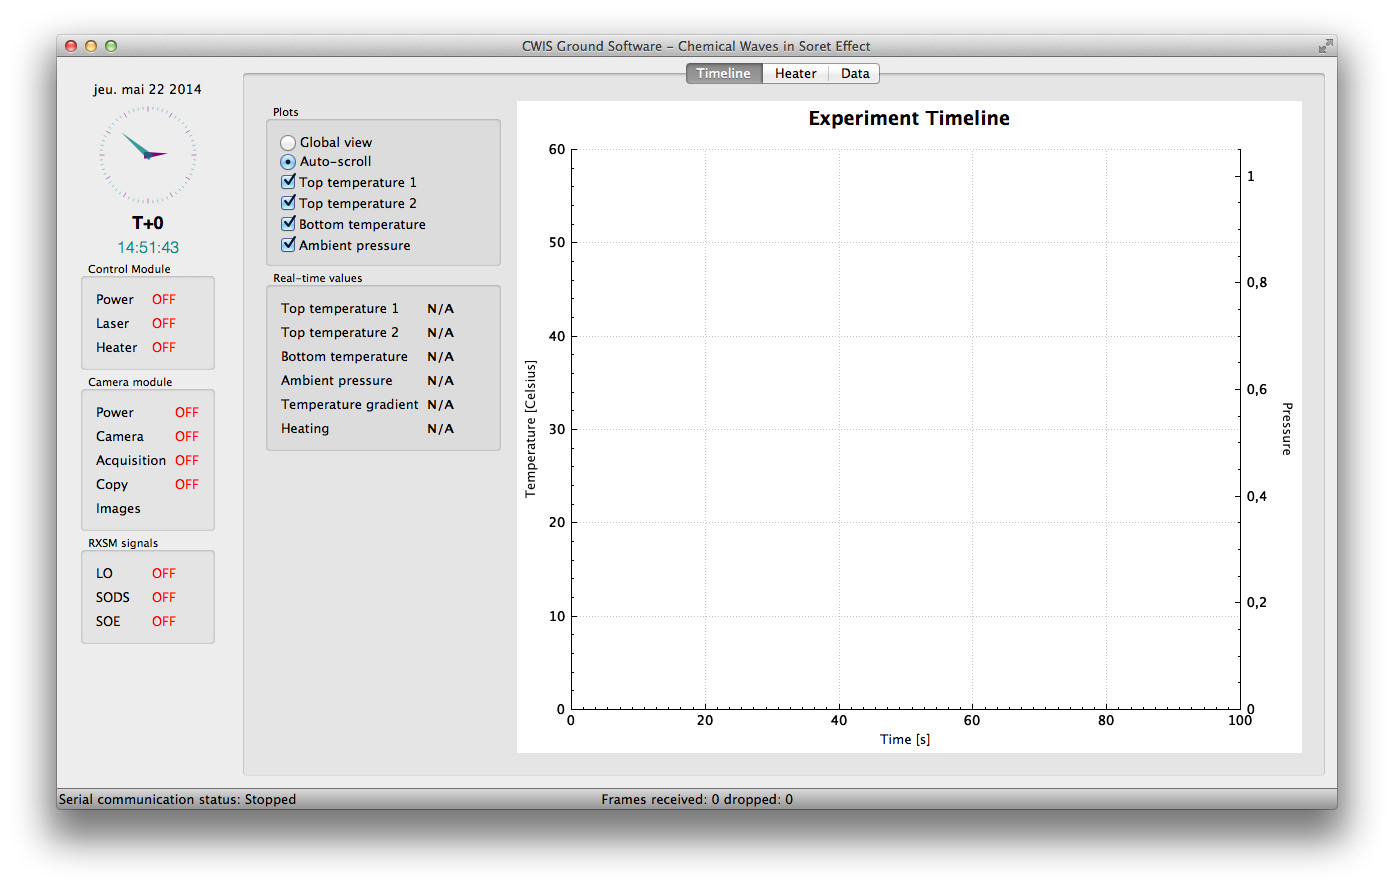
\includegraphics[width=15cm]{images/gs_main.png}
\label{image:gs_main}
\caption{Main interface of the ground software}
\end{figure}

The ground software is a graphical application developed in C++ using the Qt framework.
It provides a complete interface to analyze the data received from the experiment through downlink communication.
Furthermore, it is possible to control certain features of the experiment through this interface by sending uplink commands. \\

The ground software interface is divided in three tabs with a common side panel.
The next sections describe those in details.

\subsection{Side panel}

The side panel on the left (see figure \ref{image:gs_main} displays the current status of the experiment.
It is divided in 3 boxes: \emph{control module}, \emph{camera module} and \emph{RXSM signals}. \\

The \emph{control module} box displays the status of the microcontroller board controlling the experiment.
\begin{itemize}
\item The \textbf{Power} signal is switched on as soon as the module is ready.
\item The \textbf{Laser} signal indicates that the laser is on.
\item The \textbf{Heater} signal indicates that the heater PI control loop (and not necessarily the heater itself) is operating.
\end{itemize}

\subsection{Timeline tab}

The timeline tab (see figure \ref{image:gs_main}) allows the user to visualize the data acquired in real-time.
The main graph displays the values of the three temperature sensors and the pressure probe in real-time.
By default, this graph auto-scrolls as to display the last 100 seconds of data acquired.
You can change this behaviour by selecting \emph{Global view} in the left upper corner to display all acquired data.
By clicking on one of the plots, a tooltip displays the value and time of each data point. \\

The \emph{real-time values} box on the left displays the values for the temperature, the pressure and the heating in real-time.

\subsection{Heater tab}

\begin{figure}[!h]
\center
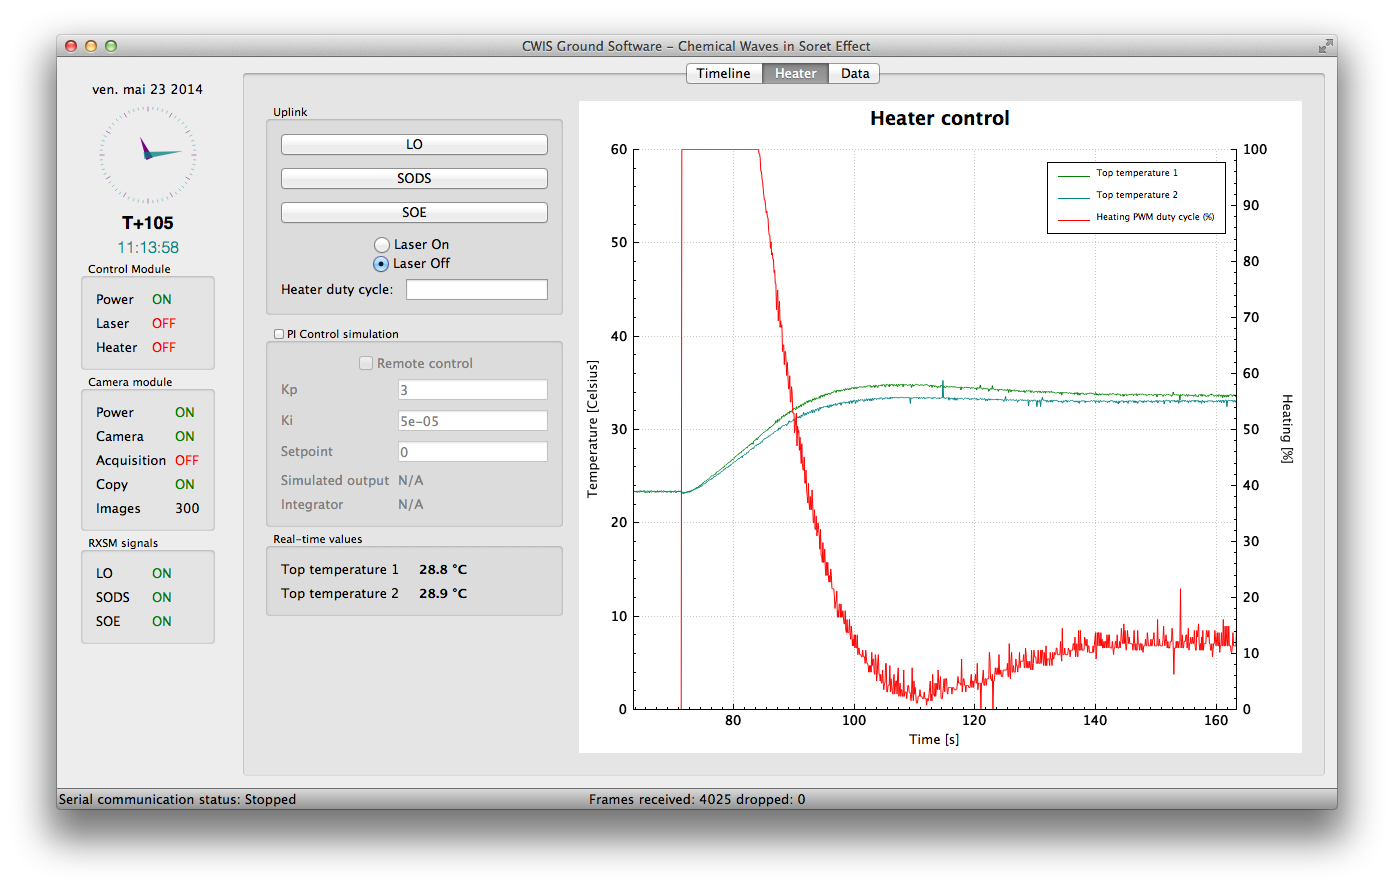
\includegraphics[width=15cm]{images/gs_heater_tab.png}
\label{image:gs_heater_tab}
\caption{Heater tab}
\end{figure}

The heater tab (figure \ref{image:gs_heater_tab}) allows the user to interact with the experiment by using the uplink channel.
It displays the top temperatures and the heating PWM.
It also integrates a PI control simulation.
See \ref{subsection:automatic_heater_control}.

\subsection{Data tab}

\begin{figure}[!h]
\center
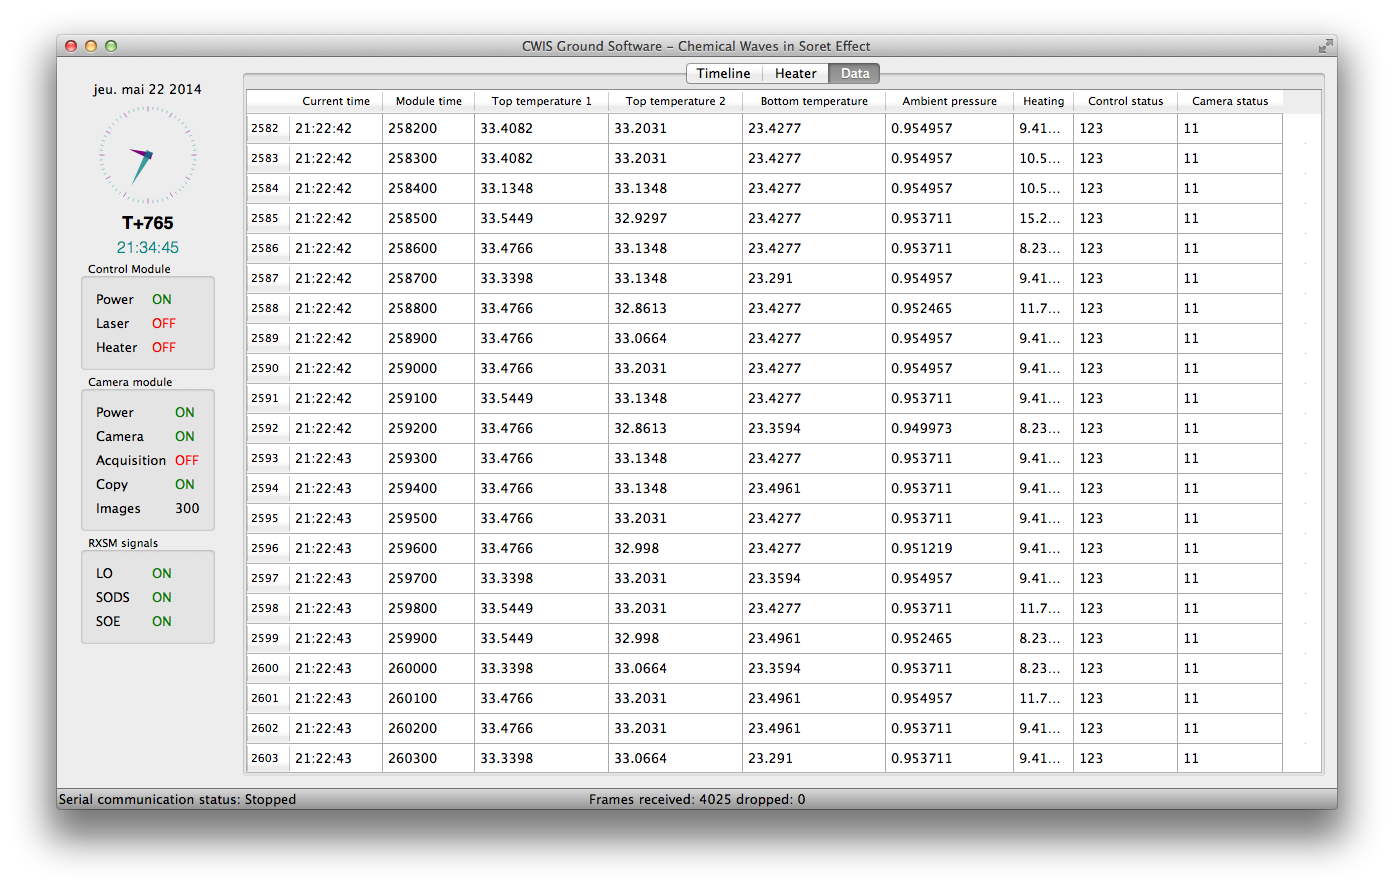
\includegraphics[width=15cm]{images/gs_data_tab.png}
\label{image:gs_data_tab}
\caption{Data tab}
\end{figure}

The data tab (figure \ref{image:gs_data_tab}) displays each data frame in its textual form.

\section{Using the ground software}

\subsection{Setting up the serial communication}

Before receiving data from the experiment, it is necessary to set up the serial port connection.
This is done using the \emph{Serial port parameters} dialog accessible from the \textbf{Serial/Configuration} menu (figure \ref{image:gs_serial_parameters}.

\begin{figure}[!h]
\center
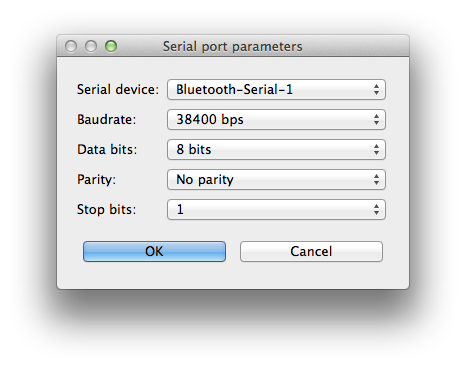
\includegraphics[scale=0.6]{images/gs_serial_parameters.png}
\label{image:gs_serial_parameters}
\caption{Serial port parameters dialog}
\end{figure}

After configuring it, you can start the serial communication using the \textbf{Serial/Start} action.
Note that the dialog pops up automatically if you try to start an unconfigured connection. \\

Please note that the serial USB adapter must be connected to the computer before starting the ground software application.

\subsection{Saving the data}

The data can be saved in two formats. The standard saving method, using the \textbf{File/Save} menu, saves the data in a formatted file for easy parsing. The second method saves the raw data from the serial frames (see \ref{section:downlink}), thus saving all information received from the module.

\subsection{Loading raw data}

By using the \textbf{File/Load raw data} menu, you can load and visualize previously acquired raw data.
Open the file and the data is automatically loaded in the different tabs.

Please note that this functionality must not be used while acquiring data.

\subsection{Basic uplink commands}

The \emph{heater tab} provides basic uplink commands to send various signals to the module.
The user can:

\begin{itemize}
\item Send the RXSM signals (LO, SODS, SOE);
\item Set the duty cycle of the heater control;
\item Switch the laser on/off.
\end{itemize}

\subsection{Automatic heater control}
\label{subsection:automatic_heater_control}

A more advanced use of the uplink channel is the automatic heater control.
The ground software integrates a simulator of the PI control loop.
It can be set to control the heater on the experiment by clicking the \emph{Remote control} checkbox.
The user can select the proportional and integral gains and the temperature setpoint.

\chapter{Serial interface}

\section{Downlink}
\label{section:downlink}

The control module sends a 24-byte wide data frame every 100 milliseconds.
This frame is described in figure \ref{image:downlink_frame}.

\begin{figure}[!h]
\center
\begin{bytefield}[bitwidth=0.6em]{64}
\bitheader{0, 8, 16, 24, 32, 40, 48, 56, 63} \\
\bitbox{16}{Synchronization} & \bitbox{16}{System time} &
\bitbox{16}{System time} & \bitbox{16}{Temperature 1}  \\
\bitbox{16}{Temperature 2} & \bitbox{16}{Temperature 3} &
\bitbox{16}{Pressure} & \bitbox{8}{Heating} & \bitbox{8}{Ctrl stat} \\
\bitbox{16}{Number of images} & \bitbox{8}{Framerate} & \bitbox{8}{Cam stat} &
\bitbox{16}{Unused} & \bitbox{16}{CRC} \\
\end{bytefield}
\label{image:downlink_frame}
\caption{Serial downlink frame}
\end{figure}

\begin{itemize}
\item \textbf{Synchronization}: Synchronization string, set to "UU". This is used to maintain synchronization between the control module and the reader application.
\item \textbf{System time}: System time of the control module, in milliseconds.
\item \textbf{Temperature}: Value read from the temperature sensors, from 0 to 1023.
\item \textbf{Pressure}: Value read from the pressure probe, from 0 to 1023.
\item \textbf{Heating}: Value of the PWM register, from 0 (0\%) to 255 (100\%).
\item \textbf{Ctrl stat}: Status of the control module.
\item \textbf{Number of images}: Number of images acquired by the camera during the experiment.
\item \textbf{Framerate}: Framerate of the camera.
\item \textbf{Cam stat}: Status of the camera module.
\item \textbf{CRC}: Cyclic Redundancy Check value. 
\end{itemize}

All values are stored in little endian (from the LSB to the MSB) except for the \textbf{Number of images} field.

\subsection{Control module status}

\begin{figure}[!h]
\begin{center}
\begin{bytefield}[bitwidth=4em]{8}
\bitheader{0-7} \\
\bitbox{1}{Unused} & \bitbox{1}{SOE} & \bitbox{1}{SODS} & \bitbox{1}{LO} &
\bitbox{1}{Heater} & \bitbox{1}{Unused} & \bitbox{1}{Laser} & \bitbox{1}{Power} \\
\end{bytefield}
\end{center}
\label{image:control_module_status}
\caption{Control module status fields}
\end{figure}

Figure \ref{image:control_module_status} describes the control module status bitfield.
The fields are self-explanatory.

\subsection{Camera module status}

\begin{figure}[!h]
\begin{center}
\begin{bytefield}[bitwidth=4em]{8}
\bitheader{0-7} \\
\bitbox{4}{Unused} &
\bitbox{1}{Copy} & \bitbox{1}{Capture} & \bitbox{1}{Camera} & \bitbox{1}{Power} \\
\end{bytefield}
\end{center}
\label{image:camera_module_status}
\caption{Camera module status fields}
\end{figure}

Figure \ref{image:camera_module_status} describes the camera module status bitfield.

\begin{itemize}
\item The \textbf{Power} bit indicates that the module has booted.
\item The \textbf{Camera} bit is set once the camera is ready for acquisition. The experiment cannot start before this bit is set.
\item The \textbf{Capture} bit indicates that the camera acquisition is ongoing.
\item The \textbf{Copy} bit is set while images are copied from RAM to persistent storage.
\end{itemize}

\section{Uplink}

All uplink frames are 4-byte wide, as shown in figure 

\begin{figure}[!h]
\begin{center}
\begin{bytefield}[bitwidth=1.1em]{32}
\bitheader{0, 8, 16, 24, 31} \\
\bitbox{8}{Command} & \bitbox{24}{Options} \\
\end{bytefield}
\end{center}
\label{image:uplink_frame}
\caption{Serial uplink frame}
\end{figure}

A lot of values are possible for those parameters; for a complete description look in the code of the ground software.

\end{document}